\documentclass[12pt]{book}

\usepackage[margin=1in]{geometry}
\usepackage{graphicx}
\graphicspath{ {../images/class1/} }
\usepackage[x11names, dvipsnames]{xcolor}
\usepackage{minted}
\usepackage{../gistex}
\usepackage{hyperref}
\usepackage[framemethod=tikz]{mdframed} % Allows defining custom boxed/framed environments

%----------------------------------------------------------------------------------------
%	INFORMATION ENVIRONMENT
%----------------------------------------------------------------------------------------
% Usage:
% \begin{info}[optional title, defaults to "Info:"]
% 	contents
% 	\end{info}

\mdfdefinestyle{info}{%
    topline=false, bottomline=false,
    leftline=false, rightline=false,
    nobreak,
    singleextra={%
        \fill[black](P-|O)circle[radius=0.4em];
        \node at(P-|O){\color{white}\scriptsize\bf T};
        \draw[very thick](P-|O)++(0,-0.8em)--(O);%--(O-|P);
    }
}

% Define a custom environment for information
\newenvironment{task}[1][Task:]{ % Set the default title to "Task:"
    \medskip
    \begin{mdframed}[style=info]
        \noindent{\textbf{#1}}
}{
    \end{mdframed}
}

\newenvironment{overview}
  {\noindent\rule{\textwidth}{0.4pt}
  \paragraph{Overview:}
  }
  {\par
  \noindent\rule{\textwidth}{0.4pt}
  }





\begin{document}
\raggedbottom
\setlength{\parskip}{0pt}

\title{CPEG472 Applied Cryptography}
\author{Andy Novicin}
\date{Spring 2019}

\maketitle

\chapter{Class 1: Hello Crypto}

\section{Introduction}

\begin{overview}
The next several katas (exercises) will have a series of tasks that walk you through the process of finding some dictionary word which has been hashed using only the result. In the process you will learn what a cryptographic hash function is, how to use codepen, cloud9, python, some great crypto libraries, basic command line scripting, and some basic coding. Most importantly you will begin to get a "gut-feel" for just how incredible modern CPUs are and why your human intuition for cryptography is not likely to be correct the first time you think about this stuff. Try to imagine the dictionary words as badly chosen passwords and think about how much "entropy" you need to make this attack infeasible.
\end{overview}

\paragraph{Peptalk:}
 This is not going to be easy, but if you stick it out you're going to have new super-powers. Every time you make progress you'll look back and wonder how you did it before. I am going to toss you into the deep-end of the pool and give you just a few google search terms to go with. Please don't get discouraged! When you are leading your team one day they will all look to you for the answers and you'll look to the internet for help. Mastery is not going to be immediate, but repeatable success will have to do. I could give you the resources to fill in all gaps but it would be large, possibly incomplete, and leave you less powerful than you would be hunting down success. I AM AVAILABLE TO HELP YOU WHERE YOU ARE THOUGH. Please don't hesitate to reach out directly.
 \newpage

\section{Kata: Hashing a dictionary word}

\begin{overview}
These two tasks will have you edit just a little bit of javascript code to get a "challenge word". If you succeed here you will have a hashed word from a standard dictionary. The next kata's will walk you through finding which word was hashed to get your word.par
\end{overview}

In this course I want you to be an effective wielder of cryptography. That means knowing how to use strong crypto schemes and knowing how to attack a weak scheme.\\

So we're going to begin by attacking SHA-512. Muah-ha-ha-ha. (You don't know what this stuff means yet but this is a top-of-the-line "Hash function". Play with this next snippet and things will start to make some sense.)

\begin{task}[CodePen 101 Task:]
Use the below codepen sample to ask my server for a random word from the scrabble dictionary to be hashed with SHA512. Now hash your own word using the input box to check that the crypto.js library's SHA512 matches PHP's SHA512 hash. (I know we haven't discussed what this means yet.)
\end{task}

\textcolor{red}{There is supposed to a JS thing here}\\

So you might now have some intuition that a "hash function" can create a long nasty looking string of letters and numbers. Also that you can feed the hash a word and get the same nasty looking string of letters and numbers. You've intuitively picked up that the hash is a repeatable scrambler of some input.

\begin{task}[CodePen 102 Task:]
Now edit the JavaScript of that pen. Change the source of the XHR request from \href{https://vip.udel.edu/crypto/sha512_with_answer.php}{\textbf{https://vip.udel.edu/crypto/sha512\_with\_answer.php}} to\\ \href{https://vip.udel.edu/crypto/sha512.php}{\textbf{https://vip.udel.edu/crypto/sha512.php}} . (Look for that first URL and remove\\ \textbf{"\_with\_answer"}.) This gives you the "hash" without telling you what word created it. Try a few random words that you think up on your own to see if you can find a match by just chance.
 \end{task}

 Now you know the main challenge of this lesson: A random word has been hashed with a strong hash function and we are trying to figure out which word it was. In the process we're going to pick up some subtle lessons about how to think in modern cryptographic terms.
\newpage

\section{Hash Functions}

\begin{overview}
This section has no action steps for you to take, it is solely here to help explain the basics of a cryptographic hash function. We will be talking more about hash functions later in the course so you don't have to know this too deeply yet. But I want to have you code sooner rather than have to wait weeks before you're brave enough. So this section is just enough that you don't stress out when you start actually coding.
\end{overview}

Now that you know the mini-challenge of lesson 1 let me tell you a bit about hash functions.\\

A hash function is something which creates a type of fingerprint from a string (or any sequence of bits). Every time anyone runs the same hash function on the same input they should get the same output.\\

Hash functions take in arbitrary length input and spit out a fixed-length output.\\

Hash functions are used as part of digital signatures, "checksums", in Message Authentication Codes (MACs), and in password storage. We'll talk about all of these thing in detail as we progress through this course. For now here are the properties of a good hash function:

\begin{itemize}
  \item Hash functions do not use a key. A key is a secret bit of information which let's you decrypt some encrypted message. In the case of hash functions it should be pretty much impossible to "decrypt"/"reverse" a hash.
  \item Crytographic hash functions should be hard to invert. That is, given $h(s)$ but not $s$, it should be computationally expensive to find $s$.
  \item Hash functions should be fast to compute.
  \item Given an input and the hash of that input, it should be hard to compute a second message which hashes to the same value. That is, given $x_1$,$h(x_1)$ it should be hard to compute $x_2$ such that $h(x_1)==h(x_2)$.
  \item It should be hard to find any two inputs that hash to the same thing.
\end{itemize}

SHA-512 is from the 2nd round of "Secure Hash Algorithms" and the output is always 512-bits. It is the most secure hash out there, although there is a 3rd iteration (SHA-3) which has just been finalized as of late 2015.
\newpage

\section{Fire up a workspace/CPU on Cloud9 or Code Anywhere}
\begin{overview}
This kata is aimed at getting you up to speed with tools that I intend to have you use on a daily basis during this course. Cloud9 is a great tool for having your own machine that you can code and command as you see fit. I also think it's valuable to have you learn command-line linux which will happen as a side-effect of working through these katas. When you are done with this kata you should have put a secret hashed word into a textfile on a new virtual machine that you control, all in your standard web browser (I prefer Chrome for this). For this course I'm going to have you do most of the heavy lifting in a scripting language. JavaScript, Python, or PHP will all fit the bill, you don't have to know those languages right now. In the next kata we will explore basic crypto in Python.
\end{overview}

Cloud9 will be a full powered development environment that we use to script/code/hack/server right in the browser.

\begin{task}[Login to Github]
If you don't have a GitHub account, go make one now.
\end{task}

\begin{task}[Cloud9 Task:]
  Cloud9 Task: You should have an email invite to cloud9 (maybe in your spam box). Now head to \href{https://c9.io}{https://c9.io} FOLLOW THE LINK FOR USERS OF THE PREVIOUS c9.io (NOT AWS) and use your github account to create a Cloud9 account. It will say the TEAM IS FULL, ignore that and click dashboard in the top right.
\end{task}

Cloud9 is a wonderful place where you can spawn up your own servers each running a well equipped Ubuntu.

\begin{task}[Create a workspace:]
Create a workspace: Spawn a workspace, name it something like sha512 , and make it a "Python"-type workspace. I've added some screenshots to help:
\end{task}


\begin{center}
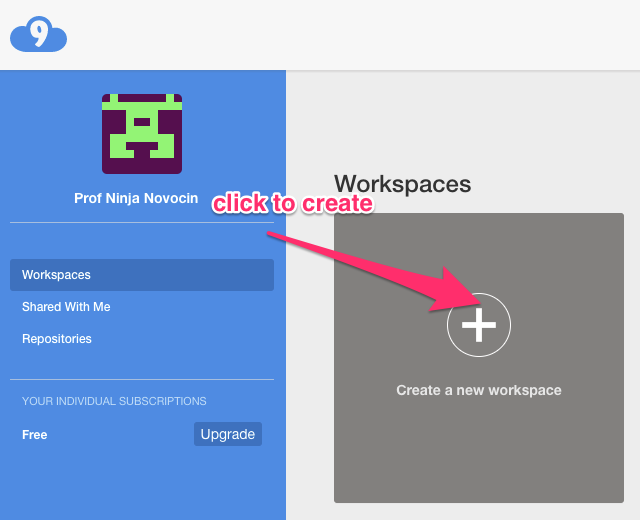
\includegraphics[width=\textwidth,height=\textheight,keepaspectratio]{create_workspace}
\end{center}

\begin{center}
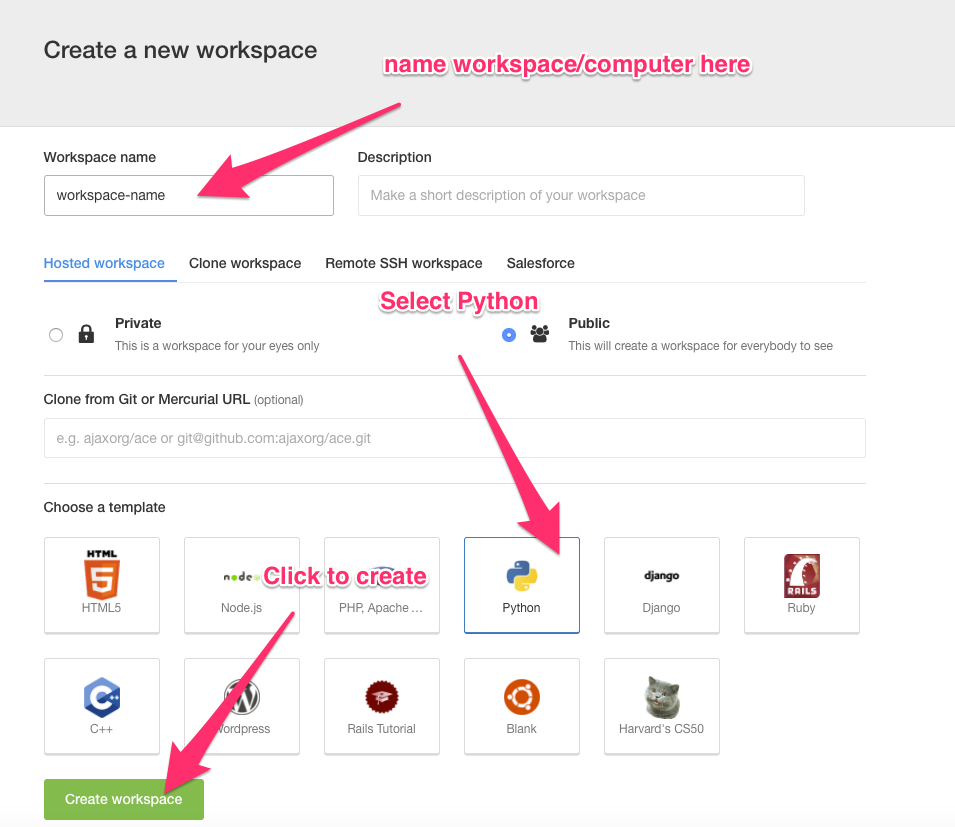
\includegraphics[width=\textwidth,height=\textheight,keepaspectratio]{Create_a_New_Workspace}
\end{center}

\begin{center}
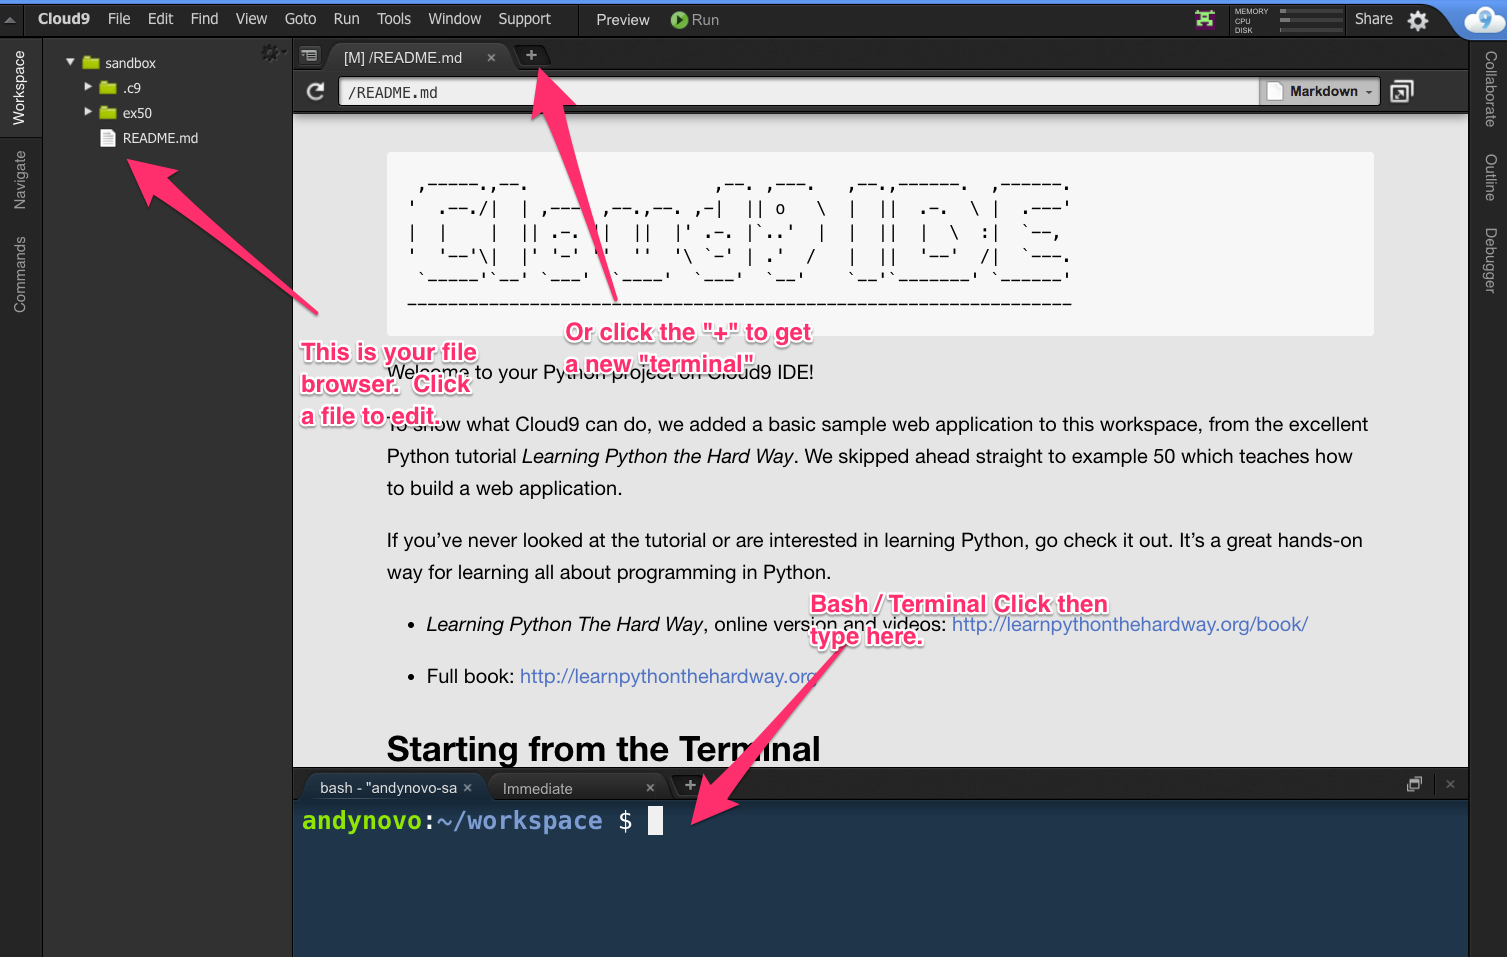
\includegraphics[width=\textwidth,height=\textheight,keepaspectratio]{Cloud9Intro}
\end{center}

\begin{task}[Get my dictionary:]
  Open your bash terminal (we'll be doing a lot of terminal work today so maybe open it wide). Use the command wget \href{https://crypto.prof.ninja/dictionary.txt}{https://crypto.prof.ninja/dictionary.txt}, that will create a file named dictionary.txt which is the source of my randomized words (scrabble legal btw).
\end{task}

\begin{center}
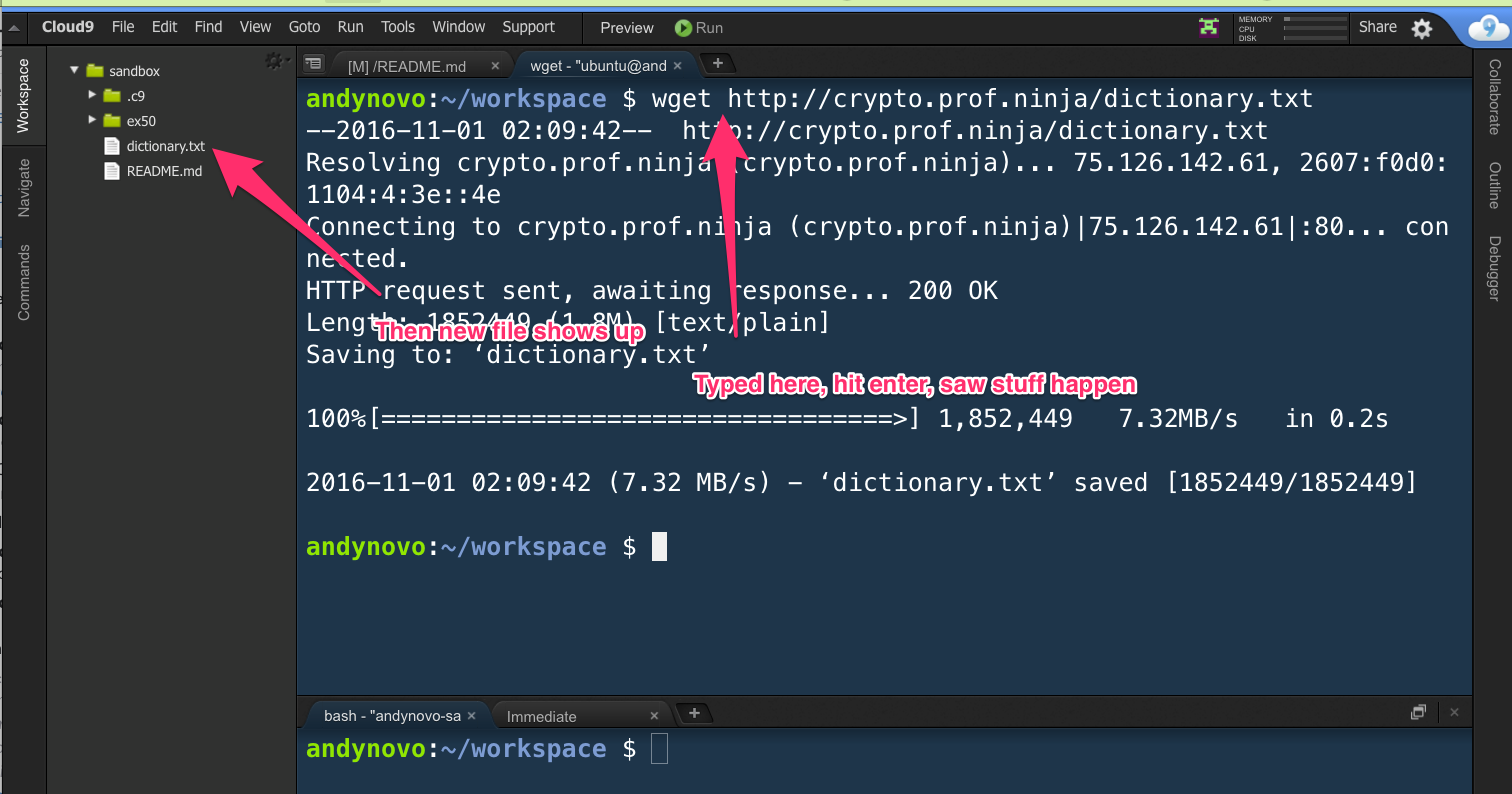
\includegraphics[width=\textwidth,height=\textheight,keepaspectratio]{terminal}
\end{center}

\begin{task}[Get yourself a target:]
  Use curl \href{https://crypto.prof.ninja/class1/sha512.php}{https://crypto.prof.ninja/class1/sha512.php} > secret to ask my server to create you a hashed word. The > secret part will send that hashed value into a file named secret . Inspect it from command line by typing more secret .
 \end{task}

 BTW, there is nothing special about Cloud9. I'm not tying you to a particular tool. Every computer of the last 30 years has a command prompt interface. If you are on an Ubuntu/Linux machine then every command I give you will work in your computer (you might have to install somethings at some point). If you are on a Mac then find terminal or iTerm inside your utilities and it will work there too. If you are on a windows machine you'll need completely different commands or to get CygWin. Learning to code in a command prompt is always very satisfying. Try hitting the up arrow, starting a command and hitting tab, etc.

 \subsection{Kata: practice BASH}
 I recommend that you practice your command line skills by mastering the basics (create a directory with mkdir, copy files with cp, move files with mv, list files with ls, remove files with rm, edit files with vi, escape a program with control+C or control+D or control+Z). Some tutorial like \href{http://www.linux-tutorial.info/modules.php?name=MContent&pageid=16}{this should help}. Remember this won't happen overnight and it's a long term investment in yourself, so don't quit or get too frustrated.

\begin{overview}
In this kata you will use the Python programming language and community built libraries to perform some basic tasks. In it you will practice using Python to read files, hash strings, and execute loops and tests. Some of you will feel more comfortable than others with these tasks. If you are nervous about using Python let me know and I'll give you some extra push. Learning Python was one of the best investments I have ever made and it's surprisingly easy to pick-up once you convince yourself that it's possible.
\end{overview}
\newpage

Python is the coolest scripting language ever:

\begin{center}
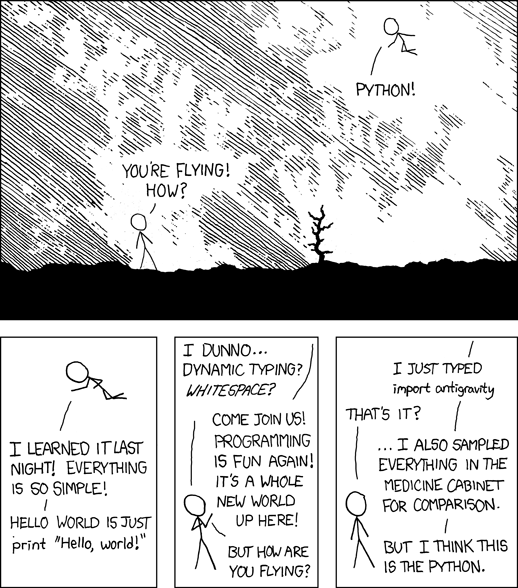
\includegraphics[scale=.5]{python}
\end{center}

Not all of you have exposure to Python. If you need to pick up a new programming language (we will use this all of the time) I highly recommend spending some time working through the first 10 project euler problems or some hacker-rank problems to get yourself up to speed. Such an exercise will be something you practice and reflect on and practice again until your confidence in Python improves.

\begin{task}[Loading a dictionary in Python:]
  So fire up a python terminal using the line ipython (enter the command in the terminal) Try to open the dictionary with something like the following three lines, one after the other:

  \begin{minted}{python}
    f=file('dictionary.txt', 'r')
    words = [word.strip() for word in f]
    f.close()
  \end{minted}
\end{task}

Note that I used ipython and not python. iPython is just python with some more user-friendliness baked in. Like tab completion on commands, the up-arrow, the ability to save your work so far, copy/paste cleanly, etc. If ipython wasn't found then you didn't start a "python" workspace, and you can just use python or make a new workspace.\\

Now you should explore the dictionary you just loaded by simply typing words[0] (first word in the dictionary) or words[-5] (fifth from the last word in the dictionary) or words[12345:12349] (a range or 4 words from the middle of the dictionary).

\begin{task}[Hash Libraries in Python:]
  Now import a library that lets you run some hash functions. Type import hashlib then in the terminal type hashlib. (that is a dot after the word hashlib) and then hit TAB (screenshot below to confirm what you're seeing). This shows you some methods in that library. Now use hashlib.sha512? to see some documentation on their sha512 method.
\end{task}

\begin{center}
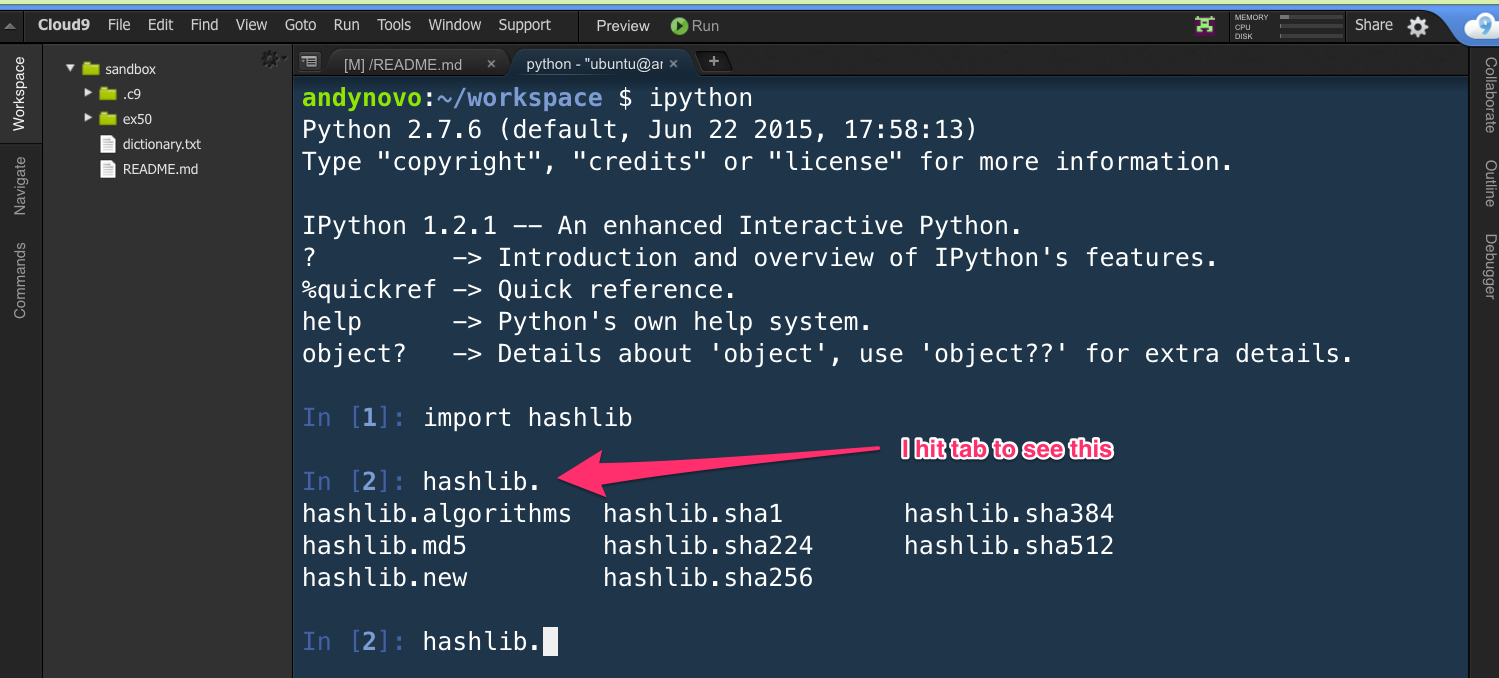
\includegraphics[width=\textwidth,height=\textheight,keepaspectratio]{ipython}
\end{center}

I'm going to try to have you run on your own for a little bit. This won't be easy, but what I'm after is that you learn how to teach yourself from documentation. There are thousands of cool modules in the world each with many cool functions. You won't find great tutorials or examples of every last function. So I want to equip you to figure out how something new works without being spoon-fed. You can google, find examples, but really start with the manual in Python. Good luck. I have a \href{https://crypto.prof.ninja/class1/kata4hint1.png}{hint link} you can look at when you need more, then finally a full solution as hidden HTML at the bottom of this task (inspect source to find it).

\begin{task}[Progress on your own:]
Now I want you to try to figure out the exact syntax to get the "hexdigest" of the phrase 'andy rocks your face off' which should hash to '64873c88f62d59e1821ac7958591dc73b4f6861b951da6ef961c33afc0d7aadb546d3515b36e5ca436cf96ad3b4046c506da3d0e234650472741afef923ee62e'.
\end{task}

The next task is asking you to take the results of the last task, apply them to every word in the array of words you have, then compare that "hexdigest" with the contents of your file "secret" (which you have to read). You might need to explore more Python if you've never done any of it before (file reading we have an example of so apply that example to the "secret" file, looping through an array is not too bad but is new for you for word in words: is how you start, getting the details right will require some care.) Good luck.

\subsection{Kata: Reverse the hash of a dictionary word}

\begin{task}
  Now see if you can figure out which word in the dictionary matches your secret word (it has a small chance of being a bad word by the way, sorry).
\end{task}

\section{What have you done?}

\begin{overview}
  This set of tasks/katas/lessons has shown you the beginnings of cryptographic action, command-line scripting, python coding, and the basics of hash functions. That's a ton for a quick lesson. It's also shown you that you will have to work hard to keep up (although it will feel easier and easier as you go forward). Don't worry, you've got the internet and optimism to protect you. Besides appreciating that I want to take a minute to reflect on the reality of how you broke the world's most secure hash algorithm without really knowing what you're doing.
\end{overview}

\subsection{Nothing protects against "pass1234"}

A hash function is one-way, it should consume something (like a password) and return impossible to reverse. Yet if you know that the password came from a universe of words that is "small" for a computer then we can "brute-force" search for something that matches the hash.\\

In this case we hashed every word in the dictionary in well under 1 second. Despite having around 200,000 words it's not enough to make the CPU sweat.

\gistex{https://gist.github.com/dc83b8d8d189b46cce7e.git}

This script will profile the cost of reversing the dictionary once. It costs around one tenth of a second for my c9 cpu to check the whole dictionary which has 187632 words (approx 200k).\\

This year has 60*60*24*366 seconds in it (approx 30 mil).

\begin{task}[Computation Task:]
  Suppose that the phrase that generated our hash digest instead was two random words, back to back, separated by a space. How long would it take try every single combination of two words?
\end{task}

\subsection{Contemplation Task:}
\begin{task}[Reverse that thinking]
  If you were to hash N random words from the dictionary (concatenated and separated by spaces), how large would N have to be in order to have this brute force attack take 1 year to guarantee success?
\end{task}

\chapter{Class 2: Proper Password Storage}

\section{Introduction}

\begin{overview}
  This lesson will walk you through some best practices for storing user passwords. While that alone might be exciting enough the real aim at this stage is to show you how to handle string encryption. That is, even if you assume that your hash algorithm is extremely powerful you must use it carefully. The ability to ballpark the cost of the brute force attacks against your scheme is one of the most valuable lessons in early crypto (or any computational endeavor).
\end{overview}

\subsection{The Password Storage Problem}

As a cryptographer you should learn to be paranoid. If you have to validate users (and you probably will have to one day) then you might end up needed to confirm their password. Imagine that you store the password in plaintext in a database or on your server somewhere. Then anyone that gets access to that file/database/server can read that user's password and go try it on all other platforms.\\

So the first rule of password storage is to NEVER STORE PLAINTEXT PASSWORDS.\\

Well this is where the Hash function comes into play. If we hash the password and store the hexdigest then a leak of that database doesn't give away the users' passwords.\\

We also saw that if the user picks a stupid password then even a hash isn't good enough to keep a brute-force attack away. So we will learn to also SALT AND STRETCH passwords (more on that soon).\\

We now have the top goal of this lesson: learn how to store a password securely. But more important is learning how to reason about the difficulty of an attacker overcoming your defenses. With that comes developing a proper level of paranoia and understanding of the power of modern computers.

\end{document}
